\documentclass[usenames,dvipsnames]{beamer}
\usepackage{../../shared/styles/custom}
\usepackage{../../shared/styles/conventions}

% Counter for pop quizzes
\newcounter{popquiz}
\setcounter{popquiz}{0}

\title{Cross-Validation}
\date{\today}
\author{Nipun Batra and teaching staff}
\institute{IIT Gandhinagar}

\begin{document}
	\maketitle

\section{Introduction to Cross-Validation}

\begin{frame}{Outline}
\tableofcontents
\end{frame}

\begin{frame}{Our General Training Flow}
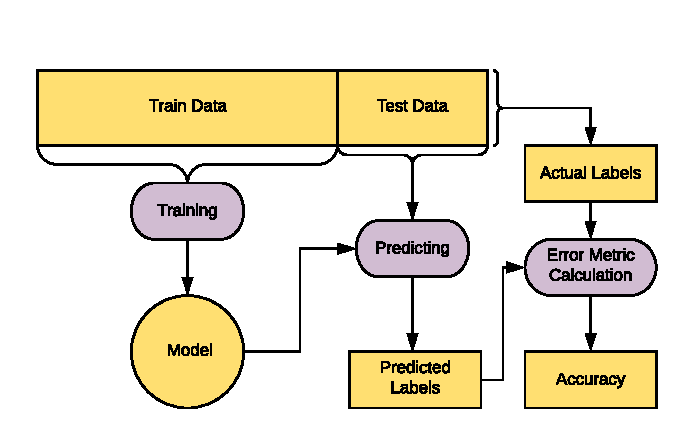
\includegraphics[width = 0.9\textwidth]{../assets/cross-validation/diagrams/general-workflow}
\begin{itemize}
	\item \pause Does not use the full dataset for training and does not test on the full dataset
	\item \pause No way to optimize hyperparameters
	\item \pause This simple train/test split has limitations we need to address
\end{itemize}
\end{frame}

\begin{frame}{Pop Quiz \stepcounter{popquiz}\#\thepopquiz}
\begin{block}{Question}
What are the main limitations of using only a single train/test split?
\end{block}
\pause
\begin{block}{Answer}
\begin{itemize}
	\item Does not utilize the full dataset for training
	\item Cannot optimize hyperparameters systematically
	\item Results depend on the particular split chosen
	\item May not get reliable performance estimates
\end{itemize}
\end{block}
\end{frame}

\section{Full Dataset Utilization}

\begin{frame}{How to use the full dataset for training?}
\begin{itemize}
	\item \pause Over multiple iterations, use different parts of the dataset for training and testing
	\item \pause Typically done via different random splits of the dataset
	\item \pause \textbf{Challenge:} How to ensure systematic evaluation?
	\item \pause May not use every data point for training or testing with random splits
	\item \pause May be computationally expensive
\end{itemize}
\end{frame}

\section{K-Fold Cross-Validation}

\begin{frame}{K-Fold Cross-Validation: Utilize Full Dataset for Testing}
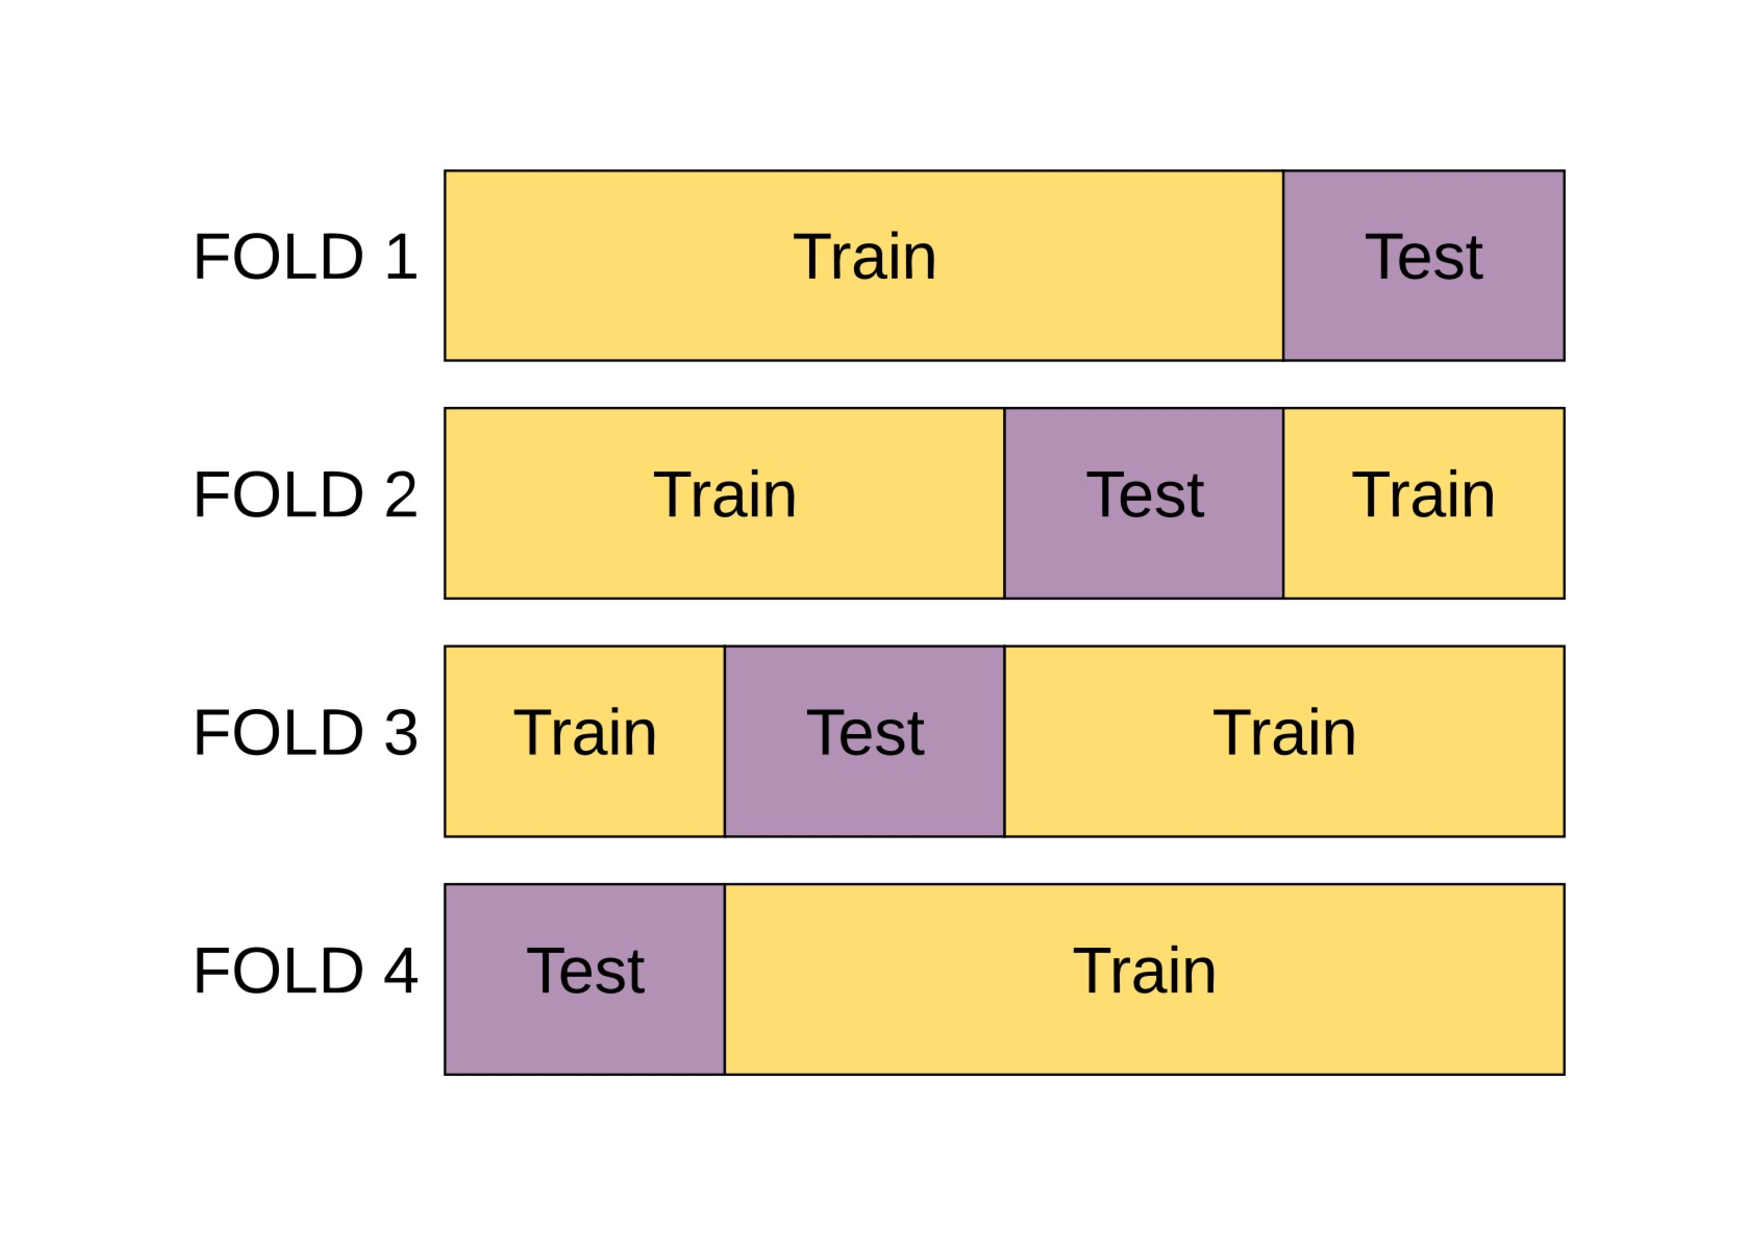
\includegraphics[width = \textwidth]{../assets/cross-validation/diagrams/cross-validation-train-test}
\pause 
\begin{itemize}
	\item Each data point is used for testing exactly once
	\item Each data point is used for training $(k-1)/k$ of the time
	\item Provides more robust performance estimates
\end{itemize}
\end{frame}

\begin{frame}{Pop Quiz \stepcounter{popquiz}\#\thepopquiz}
\begin{block}{Question}
If you have 100 data points and use 5-fold cross-validation, how many data points are used for training in each fold?
\end{block}
\pause
\begin{block}{Answer}
80 data points (4 out of 5 folds = 4/5 × 100 = 80)
\end{block}
\end{frame}

\section{Hyperparameter Optimization}

\begin{frame}{Optimizing Hyperparameters via the Validation Set}
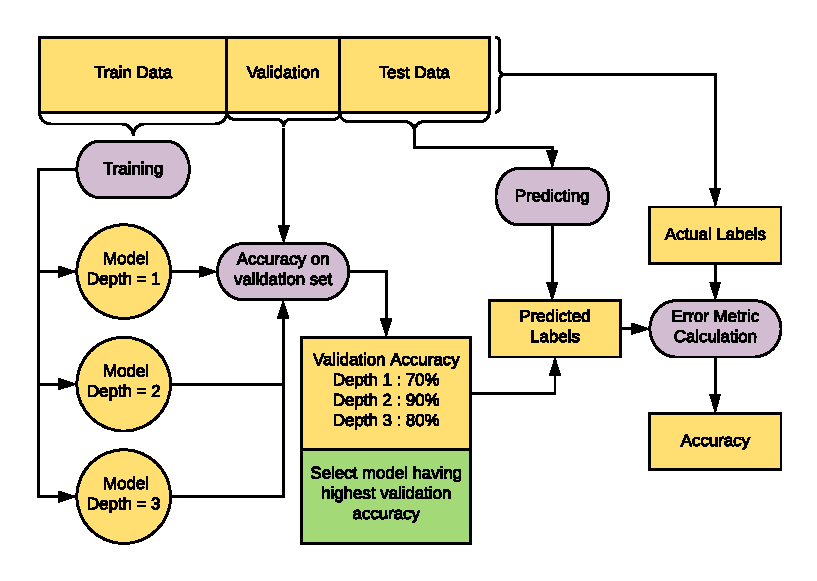
\includegraphics[width = \textwidth]{../assets/cross-validation/diagrams/validation-workflow}
\begin{itemize}
	\item \pause Validation set helps select the best hyperparameters
	\item \pause Test set remains untouched until final evaluation
	\item \pause This prevents overfitting to the test set
\end{itemize}
\end{frame}

\section{Nested Cross-Validation}

\begin{frame}{Nested Cross-Validation Process}
Divide your training set into $k$ equal parts.\\
Cyclically use 1 part as ``validation set'' and the rest for training.\\
Here $k = 4$
\begin{center}

\includegraphics[scale=0.7]{../assets/cross-validation/diagrams/cross-validation.pdf}
\end{center}
\begin{itemize}
	\item \pause Each fold provides one validation score
	\item \pause Process is systematic and exhaustive
\end{itemize}
\end{frame}

\begin{frame}{Pop Quiz \stepcounter{popquiz}\#\thepopquiz}
\begin{block}{Question}
What is the difference between simple cross-validation and nested cross-validation?
\end{block}
\pause
\begin{block}{Answer}
\begin{itemize}
	\item Simple CV: Used for model evaluation only
	\item Nested CV: Outer loop for model evaluation, inner loop for hyperparameter tuning
	\item Nested CV provides unbiased estimates when doing hyperparameter search
\end{itemize}
\end{block}
\end{frame}

\begin{frame}{Cross-Validation Results}
Average out the validation accuracy across all the folds\\
Use the hyperparameters with highest average validation accuracy\\
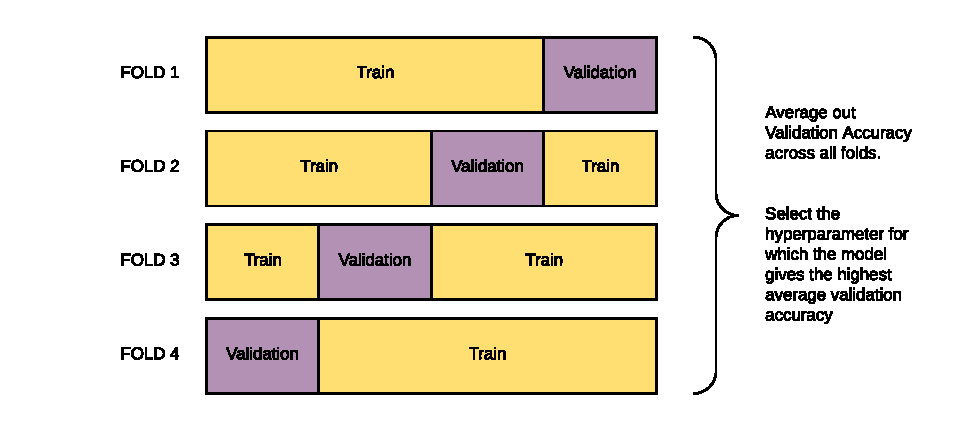
\includegraphics[width = \textwidth]{../assets/cross-validation/diagrams/cross-validation-avg.pdf}
\begin{itemize}
	\item \pause Final model is trained on entire training set
	\item \pause Standard deviation gives confidence in results
\end{itemize}
\end{frame}

\begin{frame}{Pop Quiz \stepcounter{popquiz}\#\thepopquiz}
\begin{block}{Question}
Why do we average the results across all folds instead of picking the best single fold?
\end{block}
\pause
\begin{block}{Answer}
\begin{itemize}
	\item Single fold results can be misleading due to data variance
	\item Averaging provides more robust performance estimates
	\item Reduces impact of lucky/unlucky splits
	\item Standard deviation indicates reliability of the estimate
\end{itemize}
\end{block}
\end{frame}

\section{Cross-Validation Variants}

\begin{frame}{Leave-One-Out Cross-Validation (LOOCV)}
\begin{itemize}
	\item \pause Special case where $k = n$ (number of data points)
	\item \pause Each fold uses exactly one data point for testing
	\item \pause \textbf{Advantages:}
	\begin{itemize}
		\item Maximum use of data for training
		\item Deterministic (no randomness)
	\end{itemize}
	\item \pause \textbf{Disadvantages:}
	\begin{itemize}
		\item Computationally expensive
		\item High variance in estimates
	\end{itemize}
\end{itemize}
\end{frame}

\begin{frame}{Stratified Cross-Validation}
\begin{itemize}
	\item \pause Maintains class distribution in each fold
	\item \pause Important for imbalanced datasets
	\item \pause Each fold has approximately same proportion of classes
	\item \pause \textbf{Example:} If dataset is 70\% class A, 30\% class B, each fold maintains this ratio
	\item \pause Reduces variance in performance estimates
\end{itemize}
\end{frame}

\begin{frame}{Pop Quiz \stepcounter{popquiz}\#\thepopquiz}
\begin{block}{Question}
You have a binary classification dataset with 90\% negative and 10\% positive examples. Why is stratified cross-validation important here?
\end{block}
\pause
\begin{block}{Answer}
\begin{itemize}
	\item Regular CV might create folds with very few (or zero) positive examples
	\item This would give misleading performance estimates
	\item Stratified CV ensures each fold has $\sim$10\% positive examples
	\item Results in more reliable and consistent evaluation
\end{itemize}
\end{block}
\end{frame}

\section{Time Series Cross-Validation}

\begin{frame}{Time Series Cross-Validation}
\begin{itemize}
	\item \pause Regular CV assumes data points are independent
	\item \pause Time series data has temporal dependencies
	\item \pause \textbf{Forward Chaining:} Train on past, test on future
	\item \pause \textbf{Rolling Window:} Fixed-size training window
	\item \pause \textbf{Expanding Window:} Growing training set over time
	\item \pause Never use future data to predict past!
\end{itemize}
\end{frame}

\section{Common Pitfalls and Best Practices}

\begin{frame}{Common Cross-Validation Mistakes}
\begin{itemize}
	\item \pause \textbf{Data Leakage:} Information from test set influences training
	\item \pause \textbf{Incorrect Splitting:} Not accounting for grouped data
	\item \pause \textbf{Overfitting to CV:} Too much hyperparameter tuning
	\item \pause \textbf{Wrong Preprocessing:} Scaling on entire dataset before splitting
	\item \pause \textbf{Ignoring Class Imbalance:} Not using stratified CV when needed
\end{itemize}
\end{frame}

\begin{frame}{Pop Quiz \stepcounter{popquiz}\#\thepopquiz}
\begin{block}{Question}
What's wrong with computing mean and standard deviation on the entire dataset before doing cross-validation?
\end{block}
\pause
\begin{block}{Answer}
\begin{itemize}
	\item This causes data leakage!
	\item Test fold statistics influence the training preprocessing
	\item Should compute statistics only on training folds
	\item Apply same transformation to corresponding test fold
	\item This gives more realistic performance estimates
\end{itemize}
\end{block}
\end{frame}

\section{Summary and Key Takeaways}

\begin{frame}{Cross-Validation: Key Benefits}
\begin{itemize}
	\item \pause \textbf{Better Data Utilization:} Every point used for both training and testing
	\item \pause \textbf{Robust Evaluation:} Multiple train/test splits reduce variance
	\item \pause \textbf{Hyperparameter Tuning:} Systematic way to select best parameters
	\item \pause \textbf{Model Comparison:} Fair comparison between different algorithms
	\item \pause \textbf{Confidence Estimates:} Standard deviation indicates reliability
\end{itemize}
\end{frame}

\begin{frame}{When to Use Different CV Types}
\begin{itemize}
	\item \pause \textbf{K-Fold (k=5,10):} General purpose, most common
	\item \pause \textbf{Stratified:} Imbalanced classification problems
	\item \pause \textbf{LOOCV:} Small datasets, when computational cost is acceptable
	\item \pause \textbf{Time Series CV:} Temporal data with dependencies
	\item \pause \textbf{Nested CV:} When doing extensive hyperparameter search
\end{itemize}
\end{frame}

\begin{frame}{Cross-Validation Best Practices}
\begin{itemize}
	\item \pause Always preprocess within each fold separately
	\item \pause Use stratification for classification problems
	\item \pause Report mean $\pm$ standard deviation
	\item \pause Don't overfit to cross-validation results
	\item \pause Consider computational cost vs. benefit trade-off
	\item \pause Use nested CV for unbiased hyperparameter search
\end{itemize}
\end{frame}

\begin{frame}{Next time: Ensemble Learning}
\begin{itemize}
\item How to combine various models?
\item Why combine multiple models?
\item How can we reduce bias?
\item How can we reduce variance?
\item Bootstrap aggregating (Bagging)
\item Boosting methods
\end{itemize}
\end{frame}

\end{document}
